\documentclass{standalone}
\usepackage{pgfplots}
\pgfplotsset{compat=1.18}

\begin{document}
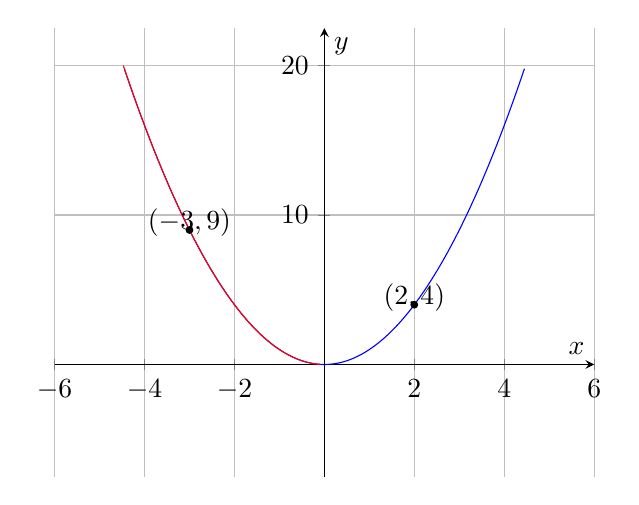
\begin{tikzpicture}
    \begin{axis}[
        axis lines=middle,
        xlabel=$x$,
        ylabel=$y$,
        ymin=-5, ymax=20,
        xmin=-5, xmax=5,
        grid=major,
        domain=-5:5,
        samples=400,
        restrict y to domain=-5:20,
        enlargelimits=true
    ]
        % Plot the entire curve in blue
        \addplot[blue] {x^2};
        
        % Highlight the negative part of the curve in red
        \addplot[red, domain=-5:-0.1] {x^2};
        
        % Add points at specific coordinates
        \node at (axis cs:-3,9) [circle, fill, inner sep=1pt]{};
        \node at (axis cs:2,4) [circle, fill, inner sep=1pt]{};
        
        % Label the points
        \node at (axis cs:-3,9.5) {$(-3, 9)$};
        \node at (axis cs:2,4.5) {$(2, 4)$};
    \end{axis}
\end{tikzpicture}
\end{document}